\begin{figure}[htpb!]
  \begin{center}
    \caption{Maternal Mortality Ratio and Women's Education}
    \label{MMRWomparl}
    \begin{subfigure}{.5\textwidth}
      \centering
      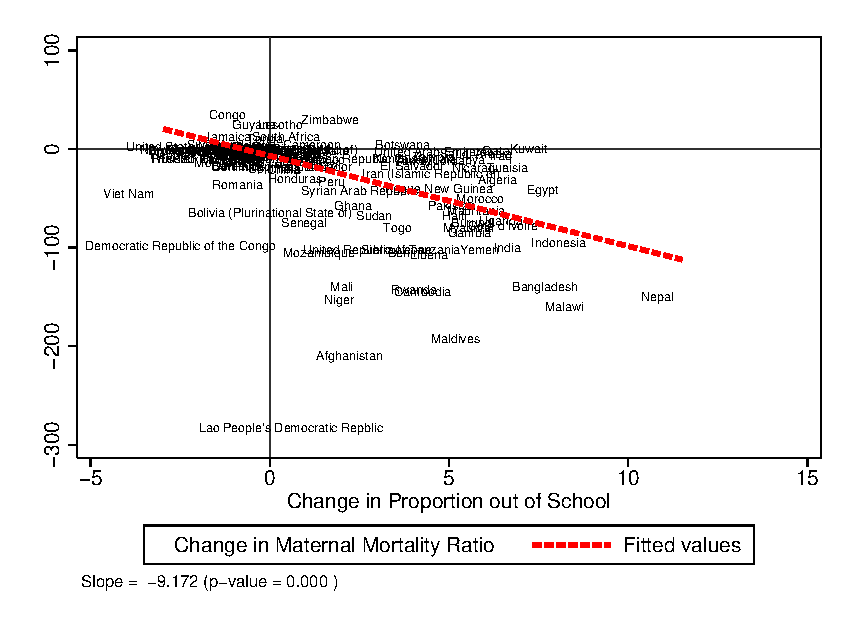
\includegraphics[scale=0.52]{\MMRfolder/Results/graphs/MMReducNDeltas.eps}
      \caption{Proportion out of School}
      \label{lowgdp}
    \end{subfigure}%
    \begin{subfigure}{.5\textwidth}
      \centering
      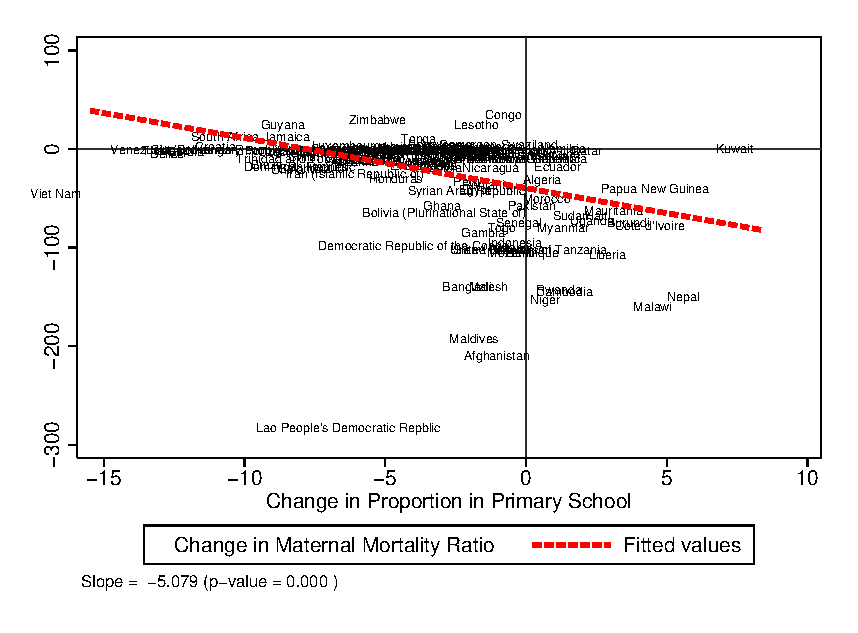
\includegraphics[scale=0.52]{\MMRfolder/Results/graphs/MMReducPDeltas.eps}
      \caption{Proportion in Primary School}
      \label{highgdp}
    \end{subfigure}
  \end{center}
  \floatfoot{\textsc{Notes to figure \ref{MMRWomparl}}: Each point
    represents the country average of $\Delta$ MMR and $\Delta$ educational indicator.
    $\Delta$ is the first difference, and is a country average over the period 1990-2010
    (the full MMR sample).  The inverse of Proportion out of School is used, so $\Delta$
    is interpreted as a \emph{reduction} in the proportion of women out of school.  Similar
    results are found when conditioning on changes in GDP per capita (see online appendix 
    figure A1).}
\end{figure}


\begin{figure}[h!]
\begin{center}
\caption{Between and Within Country Correlations: Education and MMR}
\label{fig:arrows}
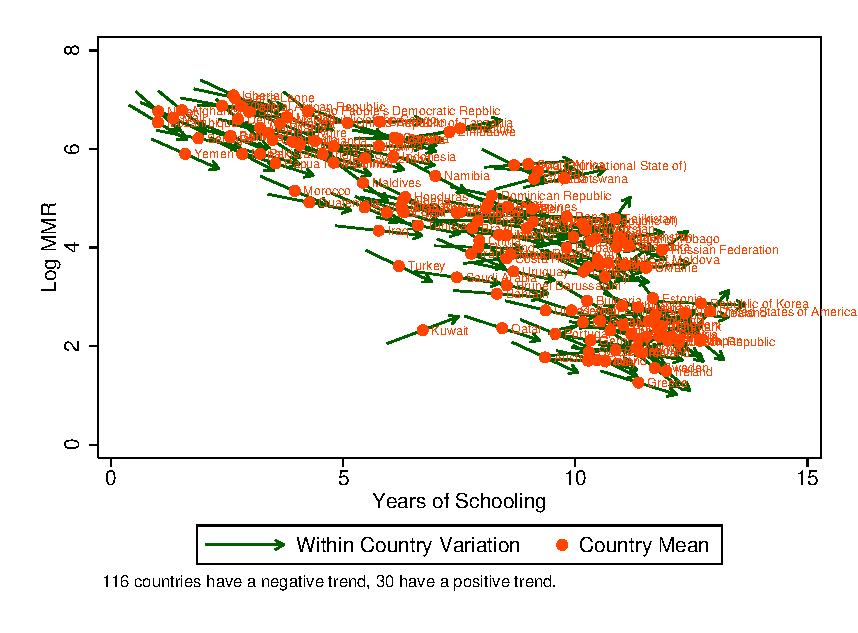
\includegraphics[scale=0.9]{\MMRfolder/Results/graphs/countries.eps} 
\end{center}
\end{figure}

\begin{figure}[h!]
\begin{center}
\caption{Effect of Primary Education on MMR by Women's Age}
\label{fig:EducAge}
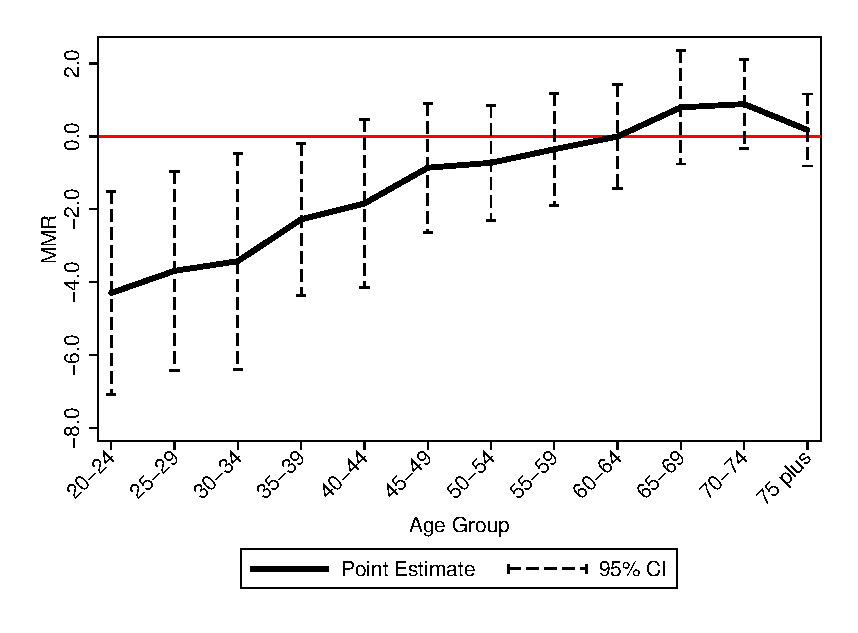
\includegraphics[scale=0.9]{\MMRfolder/Results/graphs/PrimaryAge.eps} 
\end{center}
\floatfoot{\textsc{Notes to figure \ref{fig:EducAge}}: Each point and confidence interval
  represent the results from a regression of country MMR on the Proportion of Women of that
  age with completed primary education (as per specification \ref{eqn:panel}).  The regression
  includes variables for each level of education, and the controls and country and year fixed
  effects are included as per table \ref{MMRtab:MMRpercent}.  Standard errors are clustered
  by countr. Each regression consists of the estimation sample of 108 countries and 428 year
  by country observations from table \ref{MMRtab:MMRpercent}.}
\end{figure}



\begin{figure}[htpb!]
  \begin{center}
    \caption{Maternal Mortality and Education by Year -- Nigeria}
    \label{NigeriaFig}
    \begin{subfigure}{.5\textwidth}
      \centering
      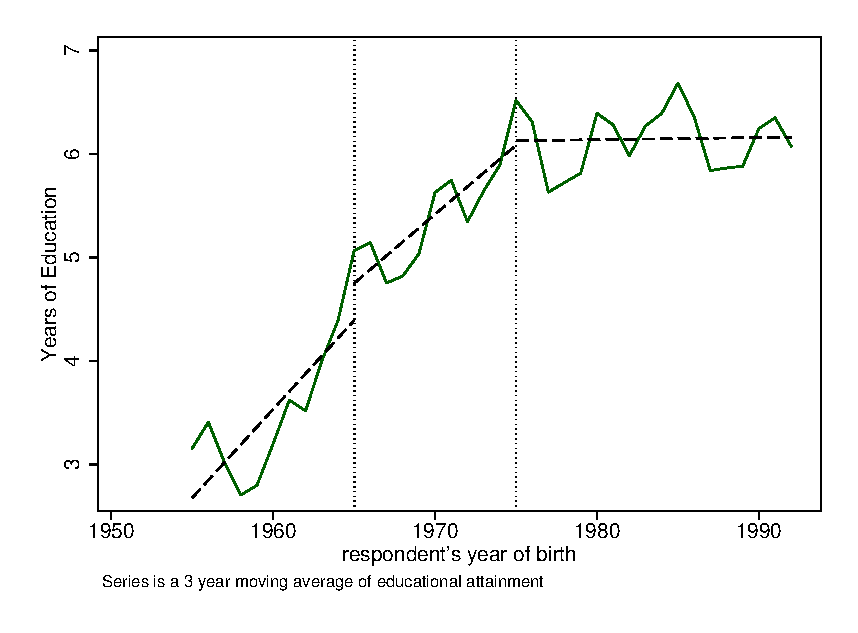
\includegraphics[scale=0.52]{\MMRfolder/Results/graphs/Nigeria_educ.eps} 
      \caption{Educational Attainment}
      \label{fig:Nigeriaeduc}
    \end{subfigure}%
    \begin{subfigure}{.5\textwidth}
      \centering
      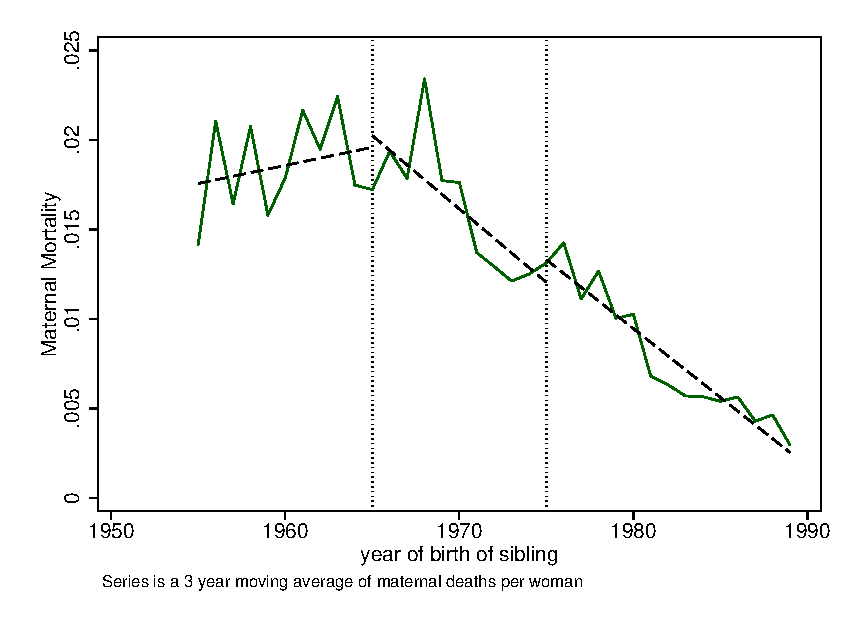
\includegraphics[scale=0.52]{\MMRfolder/Results/graphs/Nigeria_mmr.eps} 
      \caption{Maternal Mortality}
      \label{fig:Nigeriammr}
    \end{subfigure}
  \end{center}
  \floatfoot{\textsc{Notes to figure \ref{NigeriaFig}}: 3 year moving
    averages are displayed for maternal mortality and education.  The first vertical
    dotted line represents the end of the control group, and the second vertical dotted
    line represents the beginning of fully treated cohorts. Cohorts in between are
    partially treated.  Further details in the body of the text, and table 
    \ref{MMRtab:EducExp}.}
\end{figure}

\begin{figure}[htpb!]
  \begin{center}
    \caption{Maternal Mortality and Education by Year -- Kenya}
    \label{KenyaFig}
    \begin{subfigure}{.5\textwidth}
      \centering
      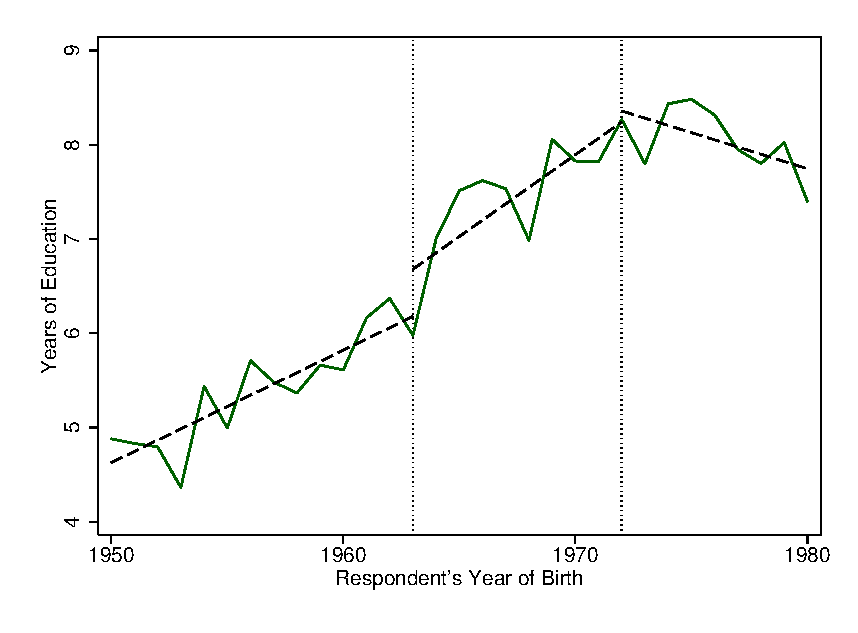
\includegraphics[scale=0.52]{\MMRfolder/Results/graphs/Kenya_educ.eps} 
      \caption{Educational Attainment}
      \label{fig:Kenyaeduc}
    \end{subfigure}%
    \begin{subfigure}{.5\textwidth}
      \centering
      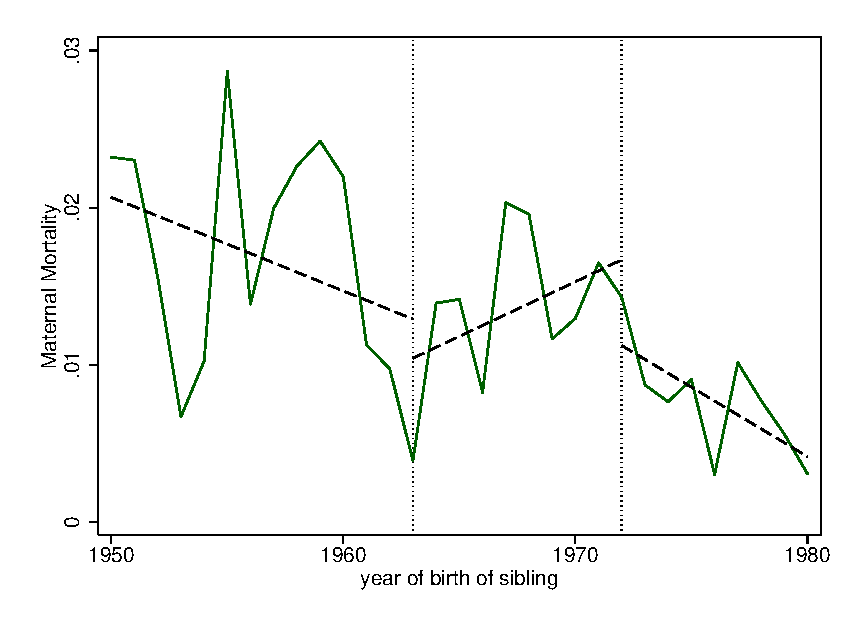
\includegraphics[scale=0.52]{\MMRfolder/Results/graphs/Kenya_mmr.eps} 
      \caption{Maternal Mortality}
      \label{fig:Kenyammr}
    \end{subfigure}
  \end{center}
  \floatfoot{\textsc{Notes to figure \ref{KenyaFig}}: The first 
    vertical dotted line represents the end of the control group, and the second 
    vertical dotted line represents the beginning of fully treated cohorts. Cohorts 
    in between are partially treated.  Further details are provided in the body of 
    the text, and in table \ref{MMRtab:EducExp}.}
\end{figure}

\begin{figure}[htpb!]
  \begin{center}
    \caption{Maternal Mortality and Education by Year -- Zimbabwe}
    \label{ZimbabweFig}
    \begin{subfigure}{.5\textwidth}
      \centering
      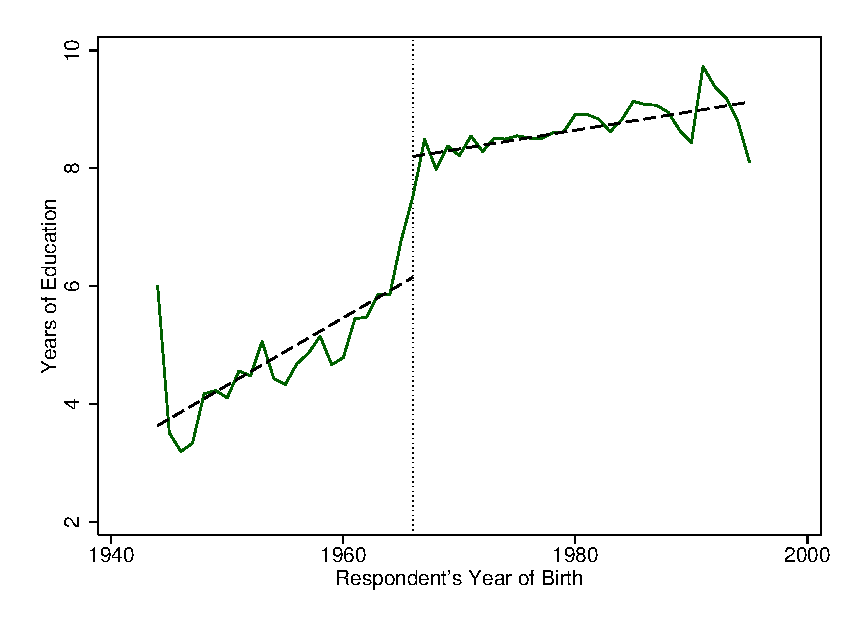
\includegraphics[scale=0.52]{\MMRfolder/Results/graphs/Zimbabwe_educ.eps} 
      \caption{Educational Attainment}
      \label{fig:Zimbabweeduc}
    \end{subfigure}%
    \begin{subfigure}{.5\textwidth}
      \centering
      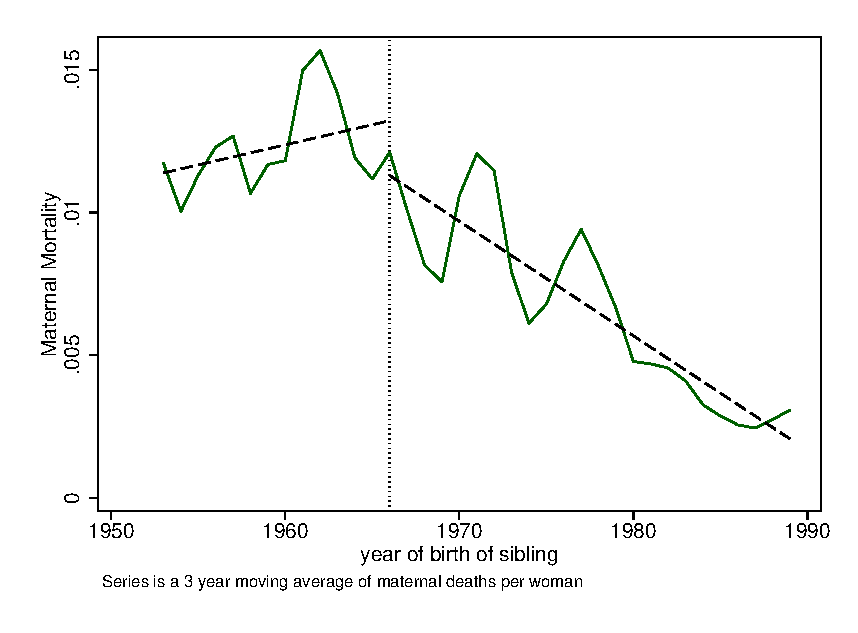
\includegraphics[scale=0.52]{\MMRfolder/Results/graphs/Zimbabwe_mmr.eps} 
      \caption{Maternal Mortality}
      \label{fig:Zimbabwemmr}
    \end{subfigure}
  \end{center}
  \floatfoot{\textsc{Notes to figure \ref{ZimbabweFig}}:
    Treatment was a one year expansion in schooling, differentially affecting
    \emph{only} the 1965/1966 cohorts.  All cohorts to the left of the vertical
    dotted line (1966 and after) are considered treated, and all cohorts to the 
    right of the line (1965 and before) are not treated. Further details are 
    provided in the body of the text, and in table \ref{MMRtab:EducExp}.}
\end{figure}


\clearpage
